\documentclass[conference]{IEEEtran}
\IEEEoverridecommandlockouts

% ---------------------------------------------------------
% Packages
% ---------------------------------------------------------
\usepackage{cite}
\usepackage{amsmath,amssymb,amsfonts}
\usepackage{algorithmic}
\usepackage{graphicx}
\usepackage{booktabs}
\usepackage{array}
\usepackage{xcolor}
\usepackage{url}
\usepackage{tikz}
\usetikzlibrary{positioning,arrows.meta,fit,backgrounds}
\usepackage[hidelinks]{hyperref}
\usepackage{balance}

\newcommand{\eg}{e.g.,\ }
\newcommand{\ie}{i.e.,\ }
\newcommand{\framework}{\textsc{McpRisk}}

\begin{document}

% ---------------------------------------------------------
% TITLE
% ---------------------------------------------------------
\title{Graduated, Two-Mode Risk Scoring\\ for AI Agent Access to Model Context Protocol Servers}

\author{
\IEEEauthorblockN{Tomer Ovadya}
\IEEEauthorblockA{Department of Software and Information Systems Engineering\\
Ben-Gurion University of the Negev\\
Beer-Sheva, Israel\\
ovadyat@post.bgu.ac.il}
\and
\IEEEauthorblockN{Asaf Shabtai}
\IEEEauthorblockA{Department of Software and Information Systems Engineering\\
Ben-Gurion University of the Negev\\
Beer-Sheva, Israel}
}

\maketitle

% ---------------------------------------------------------
% ABSTRACT
% ---------------------------------------------------------
\begin{abstract}
The Model Context Protocol (MCP) lets AI agents invoke real-world tools---file
operations, database queries, and API calls---through a uniform interface,
spawning an ecosystem of more than 67{,}000 servers. To the server that owns
those resources, every incoming agent request is a potential threat: one
malicious or misguided call can exfiltrate secrets, corrupt records, or trigger
cascading side effects. Existing MCP defenses, however, ultimately collapse to a
binary allow/deny verdict, discarding any internal severity signal before it
reaches the operator and ignoring the spectrum of risk between a safe read and a
destructive write. We present \framework, a defense-oriented framework that
produces a \emph{graduated} risk score for MCP tool invocations in two modes: a
\emph{static} score computed at design time from a server's tool registry and
asset inventory alone, and a \emph{dynamic} score computed at request time from
concrete arguments, session context, and call frequency. Scores follow an
auditable $\text{Impact}\times\text{Likelihood}\times\text{Irreversibility}$
model and are produced by a multi-stage LLM pipeline with an independent reviewer
stage and a deterministic offline fallback. We evaluate against \emph{external,
third-party} ground truth: three public MCP attack benchmarks (MCPSecBench,
MCP-SafetyBench, MSB; 150 labeled calls under the same server-as-victim threat
model), graded as an attack-detection task. The contrast is sharp: capability-only
risk frameworks (CVSS, AIVSS) sit at chance (AUC 0.52) because the attack lives in
the call's arguments, not the tool, whereas request-aware scoring---an LLM judge
over (tool, args, server), the form our dynamic mode takes---is the strongest
detector (AUC 0.68, 42\% recall at a 10\% false-positive budget). A positioning
matrix shows \framework{} is the only work that scores graduated, per-(tool, asset)
MCP risk in both a design-time and a request-time mode under this threat model and
validates it on external benchmarks. We release the framework, the baselines, and
the evaluation pipeline.
\end{abstract}

\begin{IEEEkeywords}
Model Context Protocol, AI agents, risk scoring, LLM security, access control, tool invocation.
\end{IEEEkeywords}

% ---------------------------------------------------------
% INTRODUCTION
% ---------------------------------------------------------
\section{Introduction}

The Model Context Protocol (MCP), introduced by Anthropic in late 2024,
standardizes how AI agents connect to external tool servers through a
host--client--server architecture, exposing \emph{tools}, \emph{resources},
\emph{prompts}, and \emph{sampling} as first-class primitives. Adoption has been
explosive: an empirical census counts more than 67{,}000 servers across six
public registries, exposing over 44{,}000 tools~\cite{li2025understanding_mcp}.
Each tool can read a file, mutate a database, send a message, or call a remote
API---real, often irreversible actions on resources the server owns.

This growth has outpaced security. Servers are contributed by untrusted third
parties with no mandatory review, and the protocol assumes that tool metadata is
trustworthy~\cite{hou2025mcp_landscape}. A growing literature documents the
resulting attack surface: tool poisoning that steers agent behavior through
crafted metadata~\cite{wang2025mcptox,li2026mcp_itp}, parasitic toolchains whose
danger emerges only from tool \emph{combinations}~\cite{zhao2025mind_your_server},
protocol-level exploits~\cite{maloyan2026breaking_protocol}, and covert
exfiltration through ostensibly benign logging tools~\cite{hu2026log_to_leak}.

Our vantage point is the \textbf{server as the protected asset}. Whether a
request originates from a benign-but-clumsy agent, a prompt-injected one, or an
outright malicious client, the server must decide---\emph{before execution}---
whether to let the call through. The defenses proposed so far ultimately
\emph{collapse} this decision to a binary verdict---trusted/untrusted
\cite{zhou2026mcpshield}, safe/unsafe~\cite{xing2026mcp_guard,mou2026toolsafe,xiang2025guardagent},
or allowed/blocked~\cite{shi2025progent,buhler2025agentbound}. Even systems that
reason internally over a continuous trust or confidence
score~\cite{zhou2026mcpshield} expose only the thresholded outcome, so an operator
cannot set proportionate responses. A binary gate is badly matched to reality:
reading a public README and deleting a directory of private keys are not the same
event, yet a single threshold must either over-block routine work or under-protect
crown-jewel assets.

We argue that MCP needs \emph{graduated, context-aware} risk quantification, in
the spirit of CVSS for software vulnerabilities. Recent results show that LLMs can
predict CVSS-style severity from natural-language descriptions with roughly 79\%
accuracy~\cite{jafarikhah2026description_to_score}, and that effective agent risk
signals must be \emph{dynamic}, \emph{contextual}, and
\emph{composable}~\cite{raza2025trism}. Crucially, prior graduated scoring is
performed \emph{once per static vulnerability} (CVSS) or at the level of system
governance (TRiSM), not \emph{per request} for individual MCP tool calls---which
is the granularity a gate needs.

\noindent\textbf{Contributions.} This paper makes the following contributions:
\begin{itemize}
  \item A defense-oriented threat model that fixes the MCP server as the victim
        and the agent as the threat, together with an auditable
        $\text{Impact}\times\text{Likelihood}\times\text{Irreversibility}$ risk
        model adapted from vulnerability scoring, including an explicit likelihood
        aggregator and band map (Sections~\ref{sec:threat}--\ref{sec:model}).
  \item A two-mode design---a \emph{static} design-time score over a server's
        tools and assets, and a \emph{dynamic} request-time score that can
        \emph{escalate} a call above its static ceiling (Section~\ref{sec:design}).
  \item An evaluation on \emph{external, third-party} MCP attack benchmarks framed
        as detection, showing capability-only frameworks (CVSS, AIVSS) are at chance
        while request-aware scoring detects, together with a positioning matrix
        against competing risk-scoring works (Section~\ref{sec:eval}).
\end{itemize}

% ---------------------------------------------------------
% THREAT MODEL
% ---------------------------------------------------------
\section{Threat Model}
\label{sec:threat}

Throughout this work the \textbf{MCP server is the protected asset} (the victim).
The attacker is a malicious or compromised AI agent---or the human behind it---
that sends harmful requests through the MCP protocol to damage, exfiltrate from,
or disrupt the server and the resources it manages. All attacks flow in the
\textbf{client$\rightarrow$server} direction. Concretely, the defender is a
gateway sitting in front of the server (Fig.~\ref{fig:arch}) that observes each
tool call's name, target asset, and arguments, plus whatever session history is
available, and must issue a verdict before the call executes. The defender does
not rely on anomaly detection or known-bad signatures; it instead defines,
explicitly and auditably, what makes an interaction risky.

We deliberately exclude the inverse scenario in which a malicious server attacks
the agent (\eg tool poisoning that tricks the agent into harmful behavior); that
is a complementary but distinct direction~\cite{wang2025mcptox,wang2026mindguard}.
Where poisoning is relevant here, it is only insofar as a poisoned agent
subsequently becomes a threat to the server.

% ---------------------------------------------------------
% RELATED WORK
% ---------------------------------------------------------
\section{Background and Related Work}
\label{sec:related}

We organize prior work into four threads that together motivate graduated scoring.

\noindent\textbf{Ecosystem and attack surface.}
Hou \emph{et al.}~\cite{hou2025mcp_landscape} give the first systematic analysis
of MCP, cataloging four attacker types and 16 threat scenarios over the
server lifecycle. Li and Gao~\cite{li2025understanding_mcp} quantify scale---
67{,}057 servers, 44{,}499 tools---and find leaked credentials, server-hijacking
flaws, and 408 groups of confusingly similar tool names enabling squatting; none
of the four major hosts they audit implements graduated risk assessment. Threat
taxonomies enumerate the space the defender must cover: Ferrag \emph{et al.}
\cite{ferrag2025prompt_to_protocol} span 30+ techniques across input
manipulation, model exploitation, system compromise, and protocol abuse;
Zhao \emph{et al.}~\cite{zhao2025when_mcp_servers_attack} identify 12 attack
categories over six server components; and Maloyan and
Namiot~\cite{maloyan2026breaking_protocol} show specification-level weaknesses
that amplify prompt-injection success by 23--41\%.

\noindent\textbf{Tool poisoning and parasitic attacks.}
MCPTox~\cite{wang2025mcptox} reports 72.8\% attack success for explicit tool
poisoning over 45 servers and 353 tools, while MCP-ITP~\cite{li2026mcp_itp}
achieves 84.2\% success with \emph{implicit} poisoning that evades detection at a
0.3\% rate by causing misuse of \emph{other} tools. Parasitic toolchains
\cite{zhao2025mind_your_server} reach roughly 90\% success from dangerous tool
\emph{combinations}, and Log-To-Leak~\cite{hu2026log_to_leak} weaponizes benign
logging tools for covert exfiltration---so output quality cannot serve as a safety
signal. MindGuard~\cite{wang2026mindguard} inspects the agent's internal decision
process to detect metadata-driven misuse. These results imply a risk model must
weigh tool capability, asset sensitivity, and data-flow context---not just the
surface text of a single call.

\noindent\textbf{Defenses and access control.}
MCPShield~\cite{zhou2026mcpshield} builds an adaptive ``security cognition'' by
probing servers and reasoning over execution traces, internally computing a
continuous deny signal that it then thresholds to a trusted/untrusted decision; it
defends the \emph{agent} from untrusted servers (the inverse of our direction) and
reports defense rates across several attack benchmarks. MCP-Guard
\cite{xing2026mcp_guard} cascades fast pattern matching, a fine-tuned neural
classifier, and LLM arbitration, reaching an F1 of 95.4\% on its full pipeline,
yet still emits a binary safe/unsafe verdict. ToolSafe~\cite{mou2026toolsafe} and
GuardAgent~\cite{xiang2025guardagent} likewise yield categorical decisions. On the
access-control side, Progent~\cite{shi2025progent} cuts attack success from about
39.9\% to roughly 1--2\% (and to near zero with hand-written policies) using
programmable privilege-control policies; AgentBound~\cite{buhler2025agentbound}
makes access control a first-class primitive with OS-level enforcement; and Wu
\emph{et al.}~\cite{wu2025automating_data_access} learn minimal-privilege
data-access policies. All enforce binary boundaries or expose only a thresholded
verdict, and none surfaces the \emph{degree} of risk of a permitted action.

\noindent\textbf{Risk quantification.}
Jafarikhah \emph{et al.}~\cite{jafarikhah2026description_to_score} show LLMs can
predict CVSS base metrics from descriptions ($\approx$79\% accuracy), establishing
text-based scoring as feasible---but once per static vulnerability. Raza
\emph{et al.}~\cite{raza2025trism} survey 180 papers on Trust, Risk, and Security
Management for agentic AI and themselves propose composite risk scores, but at the
level of system governance rather than per-invocation MCP tool calls. \emph{No
prior system produces a graduated, per-(tool, asset), request-instantiated risk
band for MCP gating}---the gap \framework{} fills. We position our work as a
complement that supplies the risk evidence the binary defenses above currently
discard.

% ---------------------------------------------------------
% RISK MODEL
% ---------------------------------------------------------
\section{Risk Model}
\label{sec:model}

\framework{} scores a tool interaction as a composition of three auditable
factors:
\begin{equation}
\text{Risk} \;=\; \underbrace{(\text{Sensitivity}\times\text{Blast})}_{\text{Impact}} \;\times\; \text{Likelihood} \;\times\; \text{Irreversibility}.
\label{eq:risk}
\end{equation}

\noindent\textbf{Impact} captures how bad a successful action is, along two
independent scales. \emph{Sensitivity} $s\in[1,5]$ reflects the
confidentiality/value of the asset touched, from public config (1) to regulated
data, PII, and secrets (5). \emph{Blast radius} $b\in[0,4]$ reflects how far one
action propagates, from no reach (0) through a single record (1) and a
departmental table (3) to systemic, all-users scope (4).

\noindent\textbf{Irreversibility} is instantiated by the per-tool impact level
$i\in\{1,2,3\}$: a read-only action ($i{=}1$, recoverable), a recoverable write
($i{=}2$), or a destructive/irreversible action ($i{=}3$).

\noindent\textbf{Likelihood} $L\in[0,1]$ estimates how anomalous, and thus how
plausibly malicious, the action is at runtime, from three sub-factors: baseline
deviation $d\in[0,1]$ (how unusual the action is for this principal's history),
access anomaly $a\in[0,0.9]$ (timing/volume outlier), and exposure
$e\in[0,0.9]$ (how much untrusted external content has entered the context window,
the prompt-injection surface). We aggregate them with a bounded, monotone
noisy-OR so that no single context factor saturates likelihood and history
($d$) remains the only factor that can reach $1$:
\begin{equation}
L \;=\; 1-(1-d)(1-a)(1-e), \qquad a,e\le 0.9 .
\label{eq:like}
\end{equation}

\noindent\textbf{Range and bands.} With $s\in[1,5]$, $b\in[0,4]$, $L\in[0,1]$,
$i\in\{1,2,3\}$, the raw score lies in $[0,60]$. Banding the raw number alone
makes $\sim$10\% of cells \texttt{critical}, which would halt legitimate work, so
\framework{} maps scores to four operational bands with an explicit, auditable
band map $B$ rather than a single cutoff. Writing $r=s\cdot b\cdot L\cdot i$:
\begin{equation*}
\small
B = \begin{cases}
\texttt{critical} & i{=}3 \wedge s{=}5 \wedge b{\ge}3\\
\texttt{high}     & (i{=}3 \wedge s{\ge}4)\ \vee\ r{\ge}24\ \vee\ (i{=}1\wedge s{\ge}4\wedge b{\ge}3)\\
\texttt{medium}   & r{\ge}8\ \vee\ (i{=}1\wedge s{=}5)\\
\texttt{low}      & \text{otherwise.}
\end{cases}
\end{equation*}
The map reserves \texttt{critical} for irreversible destruction of a crown-jewel
asset (sensitivity 5) at departmental-or-wider reach, keeping it rare
($\sim$1--2\% of cells). A \emph{confidentiality floor} keeps reads of secrets at
\texttt{medium} (narrow) or \texttt{high} (broad) and never \texttt{critical},
since a read changes no state but still leaks. Bands drive proportionate
responses: auto-allow, log-and-monitor, escalate-to-human, and auto-deny.

\noindent\textbf{Two modes.} The same model is evaluated at two times. In the
\emph{static} mode (design time), likelihood is pinned to its upper bound
$L{=}1$ (Eq.~\ref{eq:like} with $d{=}1$): the score is a worst-case ceiling
derived from tool and asset properties alone, answering ``which (tool, asset)
pairs on this server are inherently dangerous?'' In the \emph{dynamic} mode
(request time), the concrete arguments, session context, and frequency
instantiate $L$ and can \emph{escalate} a call above its static cell.

\noindent\textbf{Worked example.} Consider \texttt{edit\_file} on
\texttt{private\_key.pem}: $s{=}5$, $b{=}3$, $i{=}3$, $L{=}1$, so $r{=}45$ and
$B{=}\texttt{critical}$. A \texttt{read\_file} on the same asset has $i{=}1$, so
$r{=}15$ but the broad-read rule yields \texttt{high}. At request time, a
recursive/bulk read raises the parameter band, which escalates the call's final
band upward---capturing mass exfiltration that the inherent read cell alone would
miss.

% ---------------------------------------------------------
% DESIGN AND IMPLEMENTATION
% ---------------------------------------------------------
\section{Design and Implementation}
\label{sec:design}

\begin{figure}[t]
\centering
\footnotesize
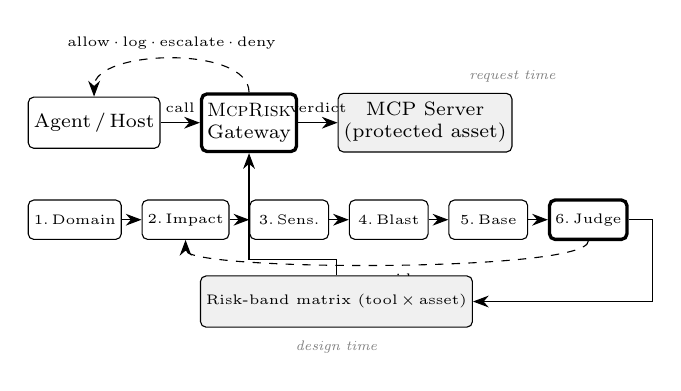
\begin{tikzpicture}[
  node distance=4.2mm and 5mm,
  box/.style={draw,rounded corners=2pt,minimum height=6.5mm,inner xsep=2pt,align=center,font=\scriptsize},
  own/.style={box,very thick},
  store/.style={box,fill=black!6},
  stage/.style={box,minimum width=10mm,minimum height=5mm,font=\tiny},
  >={Stealth[length=2mm]}
]
% --- request-time row ---
\node[box] (agent) {Agent\,/\,Host};
\node[own,right=of agent] (gw) {\framework{}\\Gateway};
\node[store,right=of gw] (srv) {MCP Server\\(protected asset)};
\draw[->] (agent) -- node[above,font=\tiny]{call} (gw);
\draw[->] (gw) -- node[above,font=\tiny]{verdict} (srv);
\draw[->,dashed] (gw.north) .. controls +(0,6mm) and +(0,6mm) .. node[above,font=\tiny]{allow\,$\cdot$\,log\,$\cdot$\,escalate\,$\cdot$\,deny} (agent.north);
% --- design-time pipeline ---
\node[stage,below=9mm of agent.south west,anchor=west] (s1) {1.\,Domain};
\node[stage,right=2.5mm of s1] (s2) {2.\,Impact};
\node[stage,right=2.5mm of s2] (s3) {3.\,Sens.};
\node[stage,right=2.5mm of s3] (s4) {4.\,Blast};
\node[stage,right=2.5mm of s4] (s5) {5.\,Base};
\node[own,right=2.5mm of s5,minimum height=5mm,font=\tiny] (s6) {6.\,Judge};
\foreach \a/\b in {s1/s2,s2/s3,s3/s4,s4/s5,s5/s6}{\draw[->] (\a)--(\b);}
\draw[->,dashed] (s6.south) .. controls +(0,-4mm) and +(0,-4mm) .. node[below,font=\tiny]{override} (s2.south);
\node[store,below=4.5mm of s3.south,xshift=6mm,minimum width=20mm,font=\tiny] (mat) {Risk-band matrix (tool\,$\times$\,asset)};
\draw[->] (s6.east) -- ++(3mm,0) |- (mat.east);
\draw[->] (mat.north) -- ++(0,2mm) -| (gw.south);
% time labels
\node[font=\tiny\itshape,gray] at ([yshift=2mm]gw.north -| srv.east) {request time};
\node[font=\tiny\itshape,gray,below=0.5mm of mat] {design time};
\end{tikzpicture}
\caption{\framework{} architecture. At \emph{design time} (bottom) a six-stage
pipeline derives a risk-band matrix from the server's \texttt{tools/list} registry
and on-disk store, with an independent judge (stage~6) overriding earlier stages.
At \emph{request time} (top) the gateway consults that matrix---and the dynamic
scorer---to gate each call before it reaches the server. Bold boxes are
\framework-owned components.}
\label{fig:arch}
\end{figure}

\framework{} is implemented in Python (3.12+) and uses a locally hosted
open-weight LLM (Qwen2.5 served through Ollama) for all judgment stages, so that
no tool metadata or asset inventory leaves the deployment.

\subsection{Static Scanner}

The static scanner runs \emph{before} a server is live and never connects to a
running server. It assembles a server description from two static sources: the
server's own saved \texttt{tools/list} registry, and the on-disk store the server
fronts (a filesystem tree, a SQL schema, or seeded channels). It then derives
every risk primitive through the six-stage pipeline of Fig.~\ref{fig:arch}:
(1)~domain inference, so later stages interpret assets in context;
(2)~tool impact ($i$); (3)~asset sensitivity ($s$); (4)~blast radius ($b$);
(5)~per-application baselines; and (6)~a judge cross-check in which an independent
reviewer re-derives every primitive from the same domain profile and
\emph{overrides} the proposer on disagreement. The pipeline then computes the cell
matrix $\text{cells}=s\times b\times L\times i$ (with $L{=}1$ at design time) and
applies the band map $B$.

Two design choices make the output trustworthy as a security artifact. First,
\textbf{nothing is hardcoded and the reference tables are never read}: if the
model is unreachable, a stage either falls back to documented deterministic
heuristics (and flags the table \texttt{needs\_human\_review}) or raises rather
than guess. Second, decoding is greedy (temperature $0$); the offline heuristic
path is bit-exact, and on our fixed model and hardware repeated LLM runs produced
identical bands, which is the property an enforcement path requires. (We do not
claim byte-identity across arbitrary GPU/driver/quantization changes.) Every judge
override is logged in a \texttt{crosscheck\_summary}, giving a reviewer a complete
decision trail.

\subsection{Dynamic Call Scorer}

At request time, the call scorer resolves an observed call to a scanned
\texttt{(tool, asset)} cell and reports that cell's score and band. Crucially, it
\textbf{never fabricates a score}: a call to a tool absent from the scan is
reported \texttt{invalid} (a misconfiguration signal), and a known tool whose
target is not a scanned cell (\eg a directory enumeration with no single-file
asset) is reported \texttt{unresolved}. When a per-tool \emph{parameter rubric} is
supplied, the scorer computes the input-parameter risk and \emph{escalates} the
inherent cell band into a final band via a monotone $\max$ (it never lowers risk),
so a large or bulk argument can raise a call above its static baseline. This
realizes the dynamic half of Eq.~\ref{eq:risk} while preserving the honesty
property that only verified cells produce numeric scores.

% ---------------------------------------------------------
% EVALUATION
% ---------------------------------------------------------
\section{Evaluation}
\label{sec:eval}

\subsection{Setup}

We built a reference corpus of seven realistic MCP servers spanning three kinds:
four filesystem servers (a generic corporate store and three domain stores---a law
firm, a media studio, and a medical clinic), two SQL servers, and one
communication (Slack) server, comprising 74 tools and a heterogeneous asset
inventory from public documents to private keys, API keys, invoices, and patient
records. Each server has a per-server, judge-reviewed \emph{design-time reference
table} held out as ground truth; across the corpus these contain 5 \texttt{critical}
cells and 52 recorded judge overrides. We \emph{evaluate the static scanner on the
five servers we have scanned to date} (the four filesystem servers and one SQL
server, 61 tools); the remaining two servers (a second SQL server and Slack) have
reference tables but were not yet scanned and so do not contribute to scanner
agreement. These design-time tables serve only as a \emph{sanity check} on the
static primitives (Sec.~\ref{sec:results}); they are LLM-reviewed and thus not fully
independent, so we do not lean on them for the headline result.

The decisive evaluation is external. We use three public, third-party MCP attack
benchmarks---MCPSecBench, MCP-SafetyBench, and MSB---comprising 150 labeled tool
calls (55 ATTACK with a 17-type attack taxonomy, 59 benign \texttt{VALID}, and
misconfiguration calls). They were authored by other groups, are entirely
independent of our framework, and share its threat model: the MCP server is the
protected asset and calls flow client$\rightarrow$server. We treat each scorer's
per-call risk as a detector of ATTACK (Sec.~\ref{sec:extdet}) and additionally
position \framework{} against competing risk-scoring works (Sec.~\ref{sec:positioning}).

\subsection{Static Sanity Check}
\label{sec:results}

\begin{table}[t]
\centering
\caption{Per-server static-scanner agreement on tool impact (read-only\,/\,
recoverable\,/\,destructive). Fractions are matching tools / total. Two further
reference servers (a SQL store and Slack) were not yet scanned.}
\label{tab:perserver}
\small
\begin{tabular}{llcc}
\toprule
\textbf{Server} & \textbf{Kind} & \textbf{Tools} & \textbf{Tool-impact} \\
\midrule
corp\_filesystem   & filesystem & 14 & 14/14 \\
law\_firm\_fs      & filesystem & 14 & 13/14 \\
media\_studio\_fs  & filesystem & 14 & 14/14 \\
medical\_clinic\_fs& filesystem & 14 & 13/14 \\
cbg\_sqlite        & SQL        & 5  & 5/5   \\
\midrule
\textbf{Total}     &            & 61 & \textbf{59/61 (97\%)} \\
\bottomrule
\end{tabular}
\end{table}

\begin{table}[t]
\centering
\caption{Static-scanner agreement by risk primitive. A \emph{cell} is one
(tool, asset-class) pair. Band/sensitivity agreement is reported on the SQL server
whose asset keys align with the reference; tool impact spans all five scanned
servers.}
\label{tab:accuracy}
\small
\begin{tabular}{lcc}
\toprule
\textbf{Primitive} & \textbf{Scope} & \textbf{Agreement} \\
\midrule
Tool impact (1--3)        & 5 servers, 61 tools & 59/61 \;(97\%) \\
Asset sensitivity (1--5)  & SQL, 7 classes      & 5/7 \;\;(71\%) \\
Composed band (exact)     & SQL, 35 cells       & 12/35 \;(34\%) \\
\bottomrule
\end{tabular}
\end{table}

\noindent\textbf{Tool impact.}
Table~\ref{tab:perserver} shows the scanner reproduces the held-out reference's
\emph{tool-impact} classification on 59 of 61 tools (97\%), and the agreement is
uniform across servers (13--14 of 14 on every filesystem server, 5/5 on SQL)
rather than carried by one easy case. This is the simplest primitive---whether a
tool reads, writes, or destroys---so we treat it as a sanity diagnostic, not the
headline result.

\noindent\textbf{Composed band.}
The fully composed band against the design-time reference agrees exactly on 34\% of
the SQL server's 35 cells (asset sensitivity 71\%; Table~\ref{tab:accuracy}). Exact
agreement is low because a band is the product of four primitives---a single-level
disagreement on any factor shifts the composed band even when each primitive is
individually close. We do not lean on this internal reference: the decisive test is
detection on \emph{external}, third-party-labeled benchmarks (Sec.~\ref{sec:extdet}).

\noindent\textbf{Error analysis.}
The scanner's residual errors are systematic and conservative rather than random.
It over-weights single-object irreversibility (rating some irreversible
writes/moves \texttt{critical}) and under-weights enumeration as an exfiltration
primitive (rating broad directory listings \texttt{low}). On SQLite it is
conservative on \emph{reads} of crown-jewel tables
(\eg \texttt{api\_keys}, \texttt{employees}), scoring them \texttt{high}/\texttt{medium}
rather than \texttt{critical}; this is a false-negative on the
security-critical cells, and is the most important limitation of the static view.
These are precisely the cases that argument-level, request-time scoring must
address, and the external detection results below (Sec.~\ref{sec:extdet}) quantify
exactly how far a capability-class-level view falls short.

\subsection{External-Benchmark Detection: Risk Scorers as Attack Detectors}
\label{sec:extdet}

The decisive test uses \emph{external, third-party ground truth}. We treat each
scorer's per-call risk as a detector of ATTACK on three public MCP benchmarks
(150 labeled calls; 55 ATTACK vs.\ 59 benign VALID) and report AUC (threshold-free
ranking quality) and recall at a 10\% false-positive budget---the way the guardrail
literature evaluates~\cite{xing2026mcp_guard,xiang2025guardagent}. We compare
capability-only frameworks (CVSS, AIVSS), which score the \emph{tool}; a
content-aware keyword detector that reads the arguments; and a request-aware
LLM judge over (tool, args, server)---the form our framework's dynamic mode takes.

\begin{table}[t]
\centering
\caption{Attack detection on external MCP benchmarks (MCPSecBench, MCP-SafetyBench,
MSB; 55 ATTACK vs.\ 59 VALID). AUC is threshold-free; recall@10\%FPR is the catch
rate at a tight false-positive budget.}
\label{tab:extdet}
\small
\begin{tabular}{lcc}
\toprule
\textbf{Scorer} & \textbf{AUC} & \textbf{Recall@10\%FPR} \\
\midrule
\textbf{LLM judge (request-aware)} & \textbf{0.68} & \textbf{42\%} \\
Keyword detector (content)         & 0.67 & 38\% \\
CVSS v3 (capability-only)          & 0.52 & \phantom{0}0\% \\
OWASP AIVSS (capability-only)      & 0.52 & \phantom{0}0\% \\
Majority / random (floor)          & $\approx$0.50 & --- \\
\bottomrule
\end{tabular}
\end{table}

Table~\ref{tab:extdet} carries the central comparison. The capability-only
frameworks are \emph{at chance} (AUC 0.52, 0\% recall at the FPR budget): on these
benchmarks the maliciousness lives in the arguments---a path-traversal
\texttt{../../etc/passwd}, an injected \texttt{<IMPORTANT>…} string, an exfiltration
payload---while CVSS and AIVSS see only the tool, which is identical across a tool's
benign and attack calls. \framework's \emph{static} band is itself
capability-class-level (Table~\ref{tab:perserver} confirms it captures tool impact),
so it shares this blind spot by construction; detecting these attacks requires
reading the request. The request-aware scorers do: the LLM judge that instantiates
our dynamic mode is the strongest detector (AUC 0.68, 42\% recall@10\%FPR),
edging the keyword detector and far above the capability frameworks, and leads on
each of the three benchmarks individually. This is external, third-party evidence
for the paper's thesis: per-call MCP risk needs request-aware scoring, not a richer
static table. We also report the honest ceiling---even the best detector reaches
only AUC 0.68, because the benchmarks include subtle tool-poisoning and rug-pull
payloads with benign-looking arguments; per-call MCP attack detection remains open.

\subsection{Positioning vs.\ Other Risk-Scoring Work}
\label{sec:positioning}

Table~\ref{tab:matrix} places \framework{} against the closest risk-scoring works.
No prior approach occupies the same cell: capability scorers (CVSS, AIVSS, the
Entra permission-risk model, description-to-CVSS) are per-vulnerability and
argument-blind; agent-safety detectors (R-Judge, AgenTRIM, AURA) emit a binary or
allow/deny verdict and are evaluated mostly by downstream task success, not
graduated risk. \framework{} is the only one that scores \emph{graduated,
per-(tool, asset) MCP invocation risk} in both a design-time and a request-time mode
under the server-as-victim threat model and validates it on external attack
benchmarks.

\begin{table}[t]
\centering
\caption{Positioning vs.\ neighbouring risk scorers. \emph{Grad.}=graduated output
(vs.\ binary); \emph{Per-call}=per-invocation granularity; \emph{Arg}=reads the
request arguments; \emph{Srv}=server-as-victim threat model; \emph{Ext.GT}=evaluated
on external labeled data.}
\label{tab:matrix}
\small
\begin{tabular}{lccccc}
\toprule
\textbf{Work} & \textbf{Grad.} & \textbf{Per-call} & \textbf{Arg} & \textbf{Srv} & \textbf{Ext.\,GT} \\
\midrule
\textbf{\framework{} (ours)} & \checkmark & \checkmark & part & \checkmark & \checkmark \\
CVSS v3 / AIVSS              & \checkmark & --        & --   & --        & \checkmark \\
Permission-risk (Entra)     & \checkmark & --        & --   & --        & \checkmark \\
AgenTRIM                    & --        & \checkmark & part & part      & -- \\
R-Judge                     & --        & \checkmark & \checkmark & part & \checkmark \\
AURA                        & \checkmark & part      & --   & --        & -- \\
MCP-RiskCue                 & \checkmark & part      & \checkmark & \checkmark & part \\
\bottomrule
\end{tabular}
\end{table}

\subsection{Threats to Validity}

The external benchmarks are modest in size (150 calls across three suites) and skew
toward tool-poisoning attacks, so the absolute AUCs are indicative rather than
definitive; we report them with a fixed-FPR operating point and a chance floor to
keep them honest. The design-time reference tables used for the static sanity check
(Tables~\ref{tab:perserver}--\ref{tab:accuracy}) were judge-reviewed by the same LLM
family the scanner uses, so they establish process---not prior---independence, and
the demo servers are author-built. Crucially, the request-aware detector we report
is a \emph{standalone LLM judge}; integrating it as \framework's dynamic stage and
evaluating the full two-mode gate end-to-end---together with larger external
benchmarks and real registry servers---is the necessary next step.

% ---------------------------------------------------------
% DISCUSSION
% ---------------------------------------------------------
\section{Discussion and Limitations}
\label{sec:discussion}

\framework{} is positioned as a complement to, not a replacement for, the binary
defenses surveyed in Section~\ref{sec:related}. A graduated score is most valuable
where those systems are weakest: deciding \emph{how} to respond once an action is
deemed non-trivially risky. By emitting a band rather than a verdict, the framework
lets an operator tune the allow/log/escalate/deny thresholds to their risk
appetite without retraining a classifier.

Two limitations bound the current design. First, the dynamic score's richness
depends on how much session context the gateway can observe at runtime; with little
visibility into agent history, the likelihood term (Eq.~\ref{eq:like}) degrades
toward its static upper bound. Second, an LLM-based scorer inherits the biases and
failure modes of its base model; the independent judge stage and the deterministic
heuristic fallback mitigate but do not eliminate this. We treat both as explicit,
audited properties rather than hidden assumptions, and the error analysis above
shows the residual failure mode (conservative scoring of crown-jewel reads) is the
one the dynamic mode is built to correct.

% ---------------------------------------------------------
% CONCLUSION
% ---------------------------------------------------------
\section{Conclusion}
\label{sec:conclusion}

We presented \framework, a defense-oriented framework that treats the MCP server
as the protected asset and produces a graduated, auditable risk score for agent
tool invocations in two modes---static at design time and dynamic at request time
---following a transparent
$\text{Impact}\times\text{Likelihood}\times\text{Irreversibility}$ model with an
explicit likelihood aggregator and band map. On external, third-party MCP attack
benchmarks framed as detection, capability-only risk frameworks (CVSS, AIVSS) sit
at chance because the attack lives in the call's arguments, while request-aware
scoring---an LLM judge over (tool, args, server), the form our dynamic mode
takes---is the strongest detector (AUC 0.68 vs.\ 0.52), and a positioning matrix
shows no prior work scores graduated, per-(tool, asset) MCP risk in both modes under
the server-as-victim model. By replacing a single allow/deny threshold with a
calibrated, operator-tunable risk band, \framework{} gives MCP servers an auditable
basis for proportionate, context-aware enforcement; integrating the request-aware
detector as the dynamic stage and evaluating the full two-mode gate on larger
external benchmarks are the immediate next steps.

% ---------------------------------------------------------
% References
% ---------------------------------------------------------
\balance
\bibliographystyle{IEEEtran}
\bibliography{refs}

\end{document}
